\chapter{Referencial Teórico}


\section{Distribuição Beta}

Segundo \cite{gomes2005} a distribuição beta é muito utilizada para modelar experimentos aleatórios cujas variáveis assumem valoreos no intervalo $(0,1)$, dada a grande flexibilidade de ajuste que seus parâmetros proporcionam. Uma variável aleatória contínua $Y$ tem distribuição beta com parâmetros $\alpha_1 > 0$ e $\alpha_2 > 0$ e sua função de densidade de probabilidade da forma

\begin{equation}
f(y)=\frac {\Gamma(\alpha_1+\alpha_2)}{\Gamma(\alpha_1)\Gamma(\alpha_2)} y^{\alpha_1-1}(1-y)^{\alpha_2-1}I_{(0,1)}(y)
\end{equation}

em que $\Gamma$ é uma função gama e $I$ representa a função indicadora.

Os parâmetros $\alpha_1$ e $\alpha_2$ são parâmetros de ajuste, por resultar em diferentes formas de densidade em $(0,1)$ através da escolha de $\alpha_1$ e $\alpha_2$. Geralmente quando $\alpha_1 = \alpha2$ as densidades são simétricas, assim, a distribuição beta pode ser vista como uma família de distribuições na Figura \ref{fig06}.


\begin{figure}[!h]
	\centering
	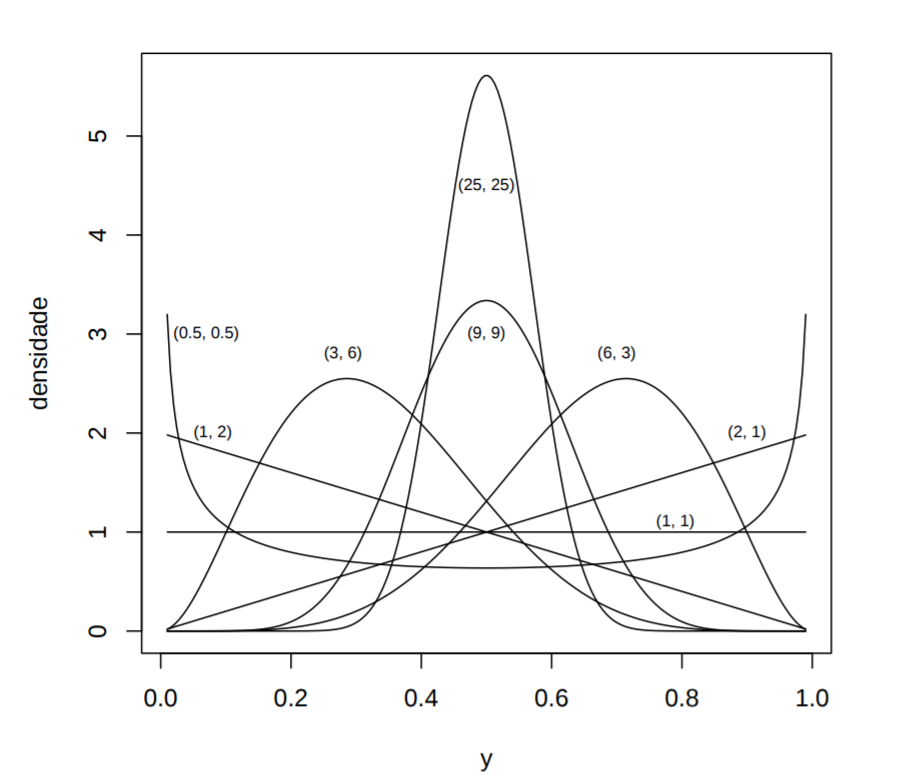
\includegraphics[keepaspectratio=true,scale=0.3]{figuras/dist-beta1.png}
	\caption{Gráfico de densidade beta para diferentes valores de $\alpha_1$ e $\alpha_2$}
	Fonte: \cite{gomes2005}
	\label{fig06}
\end{figure}


Ao se fixar $\alpha_2$, no lado esquerdo da \ref{fig07}, é obtido a variação de densidade beta para diferentes valores de $\alpha_1$; O mesmo acontece ao se fixar o $\alpha_1$, no lado direito da \ref{fig07}, é obtido a variação de densidade beta para diferentes valores de $\alpha_2$. Ao permutar $\alpha_1$ e $\alpha_2$ ocorre uma reflexão em torno da reta $y = 0,5$, devido à expressão da densidade como função de $y$ e $y-1$. 

Se $Y$ tem distribuição beta, a esperança é dada por

$$ E(Y) = \frac {\alpha_1}{\alpha_1 + \alpha_2} $$

e a variância é dada por

$$ Var(Y) = \frac{\alpha_1\alpha_2}{(\alpha_1+\alpha_2)^2(\alpha_1+\alpha_2+1)} $$


\begin{figure}[!h]
	\centering
	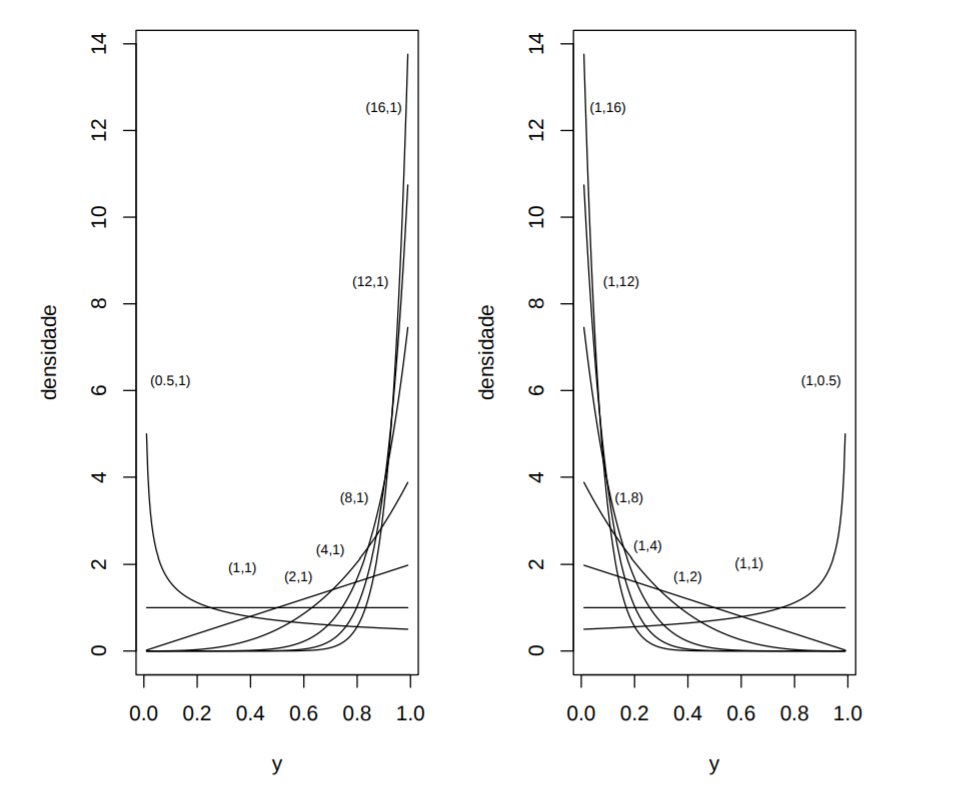
\includegraphics[keepaspectratio=true,scale=0.4]{figuras/dist-beta2.png}
	\caption{Gráfico de densidade beta para diferentes valores de $\alpha_1$ e $\alpha_2$, fixando $\alpha_2 = 1$ (esquerda) e $\alpha_1 = 1$ (direita)}
	Fonte: \cite{gomes2005}
	\label{fig07}
\end{figure}


Através da equação da variância pode-se observar que a variabilidade de $Y$ diminui à medida que se aumenta os valores dos dois parâmetro; pode ser visto na Figura \ref{fig06} quando as distribuições são simétricas.


\section{Distribuição Dirichlet}


Segundo \apud{lovelace1998}{barbosa2018} a distribuição de Dirichlet é uma família de distribuições de probabilidade multivariada contínuas, parametrizada por um vetor de parâmetros $\alpha$, denotada por $Dir(\alpha)$. É uma generalização multivariada da distribuição Beta, podendo ser empregada no estudo da distribuição de vetores aleatórios, cuja as variáveis aleatórias estejam compreendidas no intervalo (0,1) e a soma é igual a 1.

Seja $\textbf{p}$ um vetor aleatório cujos elementos somam 1, de modo que $p_{k}$ represente a proporção do item \textit{k}. De acordo \cite{minka2000}, sob o modelo de Dirichlet com o vetor de parâmetros $\alpha$, a densidade de probabilidade em $\textbf{p}$ é


\begin{equation}
p(\boldsymbol {p}) \sim \mathcal{D}(\alpha_{1},\dots,\alpha_{k}) = \frac {\Gamma(\sum_{k} \alpha_{k})}{\prod_{k}\Gamma(\alpha_{k})} \prod_{k} p_{k}^{\alpha_{k}-1}
\end{equation}


Onde $p_{k} > 0$ 
\begin{equation}
\sum_{k} p_{k} = 1
\end{equation}    

O parâmetro $\alpha$ é um vetor $k$ com componentes $\alpha_i > 0$, e onde $\Gamma(x)$ é a função Gamma \cite{blei2003}.
Os parâmetros $\alpha$ são estritamente positivos e um fato importante é que as densidades marginais da distribuição Dirichlet são beta \cite{gomes2005}.

Seja $\phi = \sum_{i=1}^{p} \alpha_i$


\begin{equation}
E(Y_i) = \frac{\alpha_i}{\phi}, \quad i = 1, \dots, p-1,
\end{equation} 

\begin{equation} \label{dir:var}
Var(Y_i) = \frac{\alpha_i(\phi-\alpha_i)}{\phi^2(\phi+1)}, \quad i = 1, \dots, p-1,
\end{equation} 



Segundo \cite{blei2003} uma variável aleatória Dirichlet $k$-dimensional $\theta$ pode assumir valores no $(k-1)$-simplex (um vetor-$k$ $\theta$ encontra-se no $(k-1)$-simplex se $\theta_i \geq 0$,
$\sum_{i=1}^{k} \theta_i =1)$. 
O Dirichlet é uma distribuição conveniente no simplex - está na família exponencial, tem estatísticas suficientes de dimensão finita e é conjugada à distribuição multinomial.


Para a maior compreensão da distribuição de Dirichlet, o trabalho de visualização foi replicado com base em \cite{liu2019}. Com $k=3$ e $2$-simplex, $k=(\alpha_1, \alpha_2, \alpha_3)$. 


\begin{figure}[!h]
	\centering
	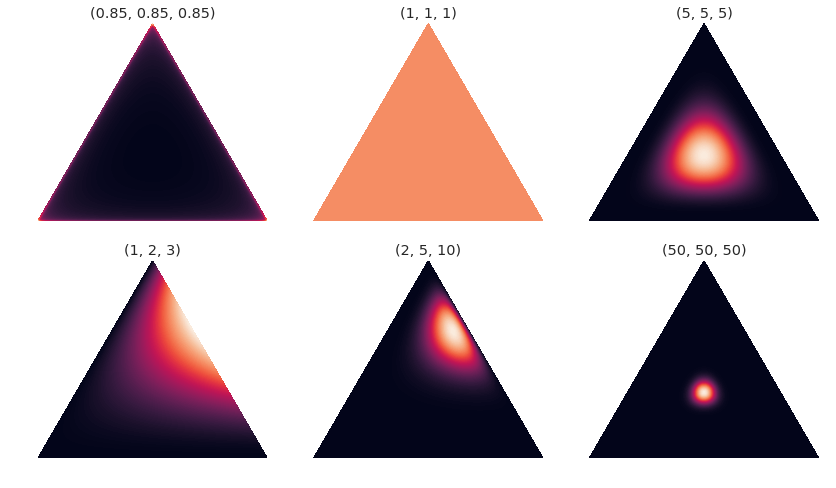
\includegraphics[keepaspectratio=true,scale=0.35]{figuras/dist-diri-simplex.png}
	\caption{Distribuição de $\alpha_1$, $\alpha_2$ e $\alpha_3$ no 2-simplex}
	Fonte: do próprio autor
	\label{fig08}
\end{figure}


Em distribuições simétricas para valores de $\alpha<1$, a distruibuição se concentra nos cantos e ao longo dos limites do simplex. No caso de $\alpha=1$, $k=(1,1,1)$, produz uma distribuição uniforme, onde todos os pontos do simplex são igualmente prováveis. Para valores $\alpha>1$, a distribuição tende para o centro do simplex, como pode ser visto na Figura \ref{fig08}. Conforme $\alpha_i$ aumenta, a distribuição se torna mais concentrada em torno do centro do simplex. 


\begin{figure}[!h]
	\centering
	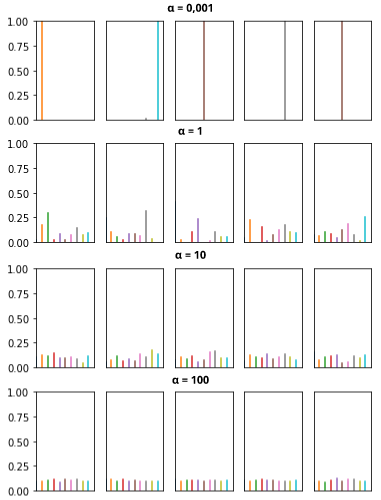
\includegraphics[keepaspectratio=true,scale=0.7]{figuras/dist-diri-var.png}
	\caption{Distribuição Dirichlet com $i=10$ e variações de $\alpha$ = 0,001, 1, 10 e 100 }
	Fonte: do próprio autor
	\label{fig09}
\end{figure}

Como especificado na Equação \ref{dir:var}, é possível observar que quanto maior o valor de $\alpha_i$, menor a variância na Figura \ref{fig09} que contém um conjunto de cinco distribuições Dirichlet, com $i=10$ e todos os $\alpha$ são iguais. Para cada distribuição a $\sum_{i=1}^{10} \alpha_i = 1$.


\section{Aprendizado de Máquina}

Aprendizado de Máquina (AM) é uma área de Inteligência Artificial (IA) cujo objetivo é o desenvolvimento de técnicas computacionais sobre o aprendizado bem como a construção de sistemas capazes de adquirir conhecimento de forma automática. Um sistema de aprendizado é um programa de computador que toma decisões baseado em experiências acumuladas através da solução bem sucedidade de problema anteriories \cite{monard2003}. 

\cite{mitchell1997} define que um programa computacional aprende a partir da experiencia E, em relação a uma classe de tarefas T, com medida de desempenho P, se seu desempenho nas tarefas T, medida por P, melhora com a experiência E.


A indução é a forma de inferência lógica que permite obter conclusões genéricas sobre um
conjunto particular de exemplos. Ela é caracterizada como o raciocínio que se origina em um conceito específico e o generaliza, ou seja, da parte para o todo. É um dos principais métodos utilizados para derivar conhecimento novo e predizer eventos futuros. 


O aprendizado indutivo é efetuado a partir de raciocínio sobre exemplos fornecidos por um processo externo ao sistema de aprendizado. O aprendizado indutivo pode ser dividido em supervisionado e não-supervisionado. 

Os algoritmos de AM são utilizados para detecção de fraudes, análise de crédito, sistemas de recomendação, mecanismos de buscas, entre outros.



\subsection{Aprendizado Supervisionada}


No aprendizado supervisionado é fornecido ao algoritmo de aprendizado, ou indutor, um conjunto de exemplos de treinamento para os quais o rótulo (\textit{label}) da classe associada é conhecido.

Em geral, cada exemplo é descrito por um vetor de valores de características, ou atributos, e o rótulo da classe associada. O objetivo do algoritmo de indução é construir um classificador que possa determinar corretamente a classe de novos exemplos ainda não rotulados, ou seja, exemplos que não tenham o rótulo da classe. Para rótulos de classe discretos, esse problema é conhecido como classificação e para valores contínuos como regressão. \cite{monard2003}



\subsection{Aprendizado Não Supervisionada}

Já no aprendizado não-supervisionado, o indutor analisa os exemplos fornecidos e tenta determinar se alguns deles podem ser agrupados de alguma maneira, formando agrupamentos ou \textit{clusters}. Após a determinação dos agrupamentos, normalmente, é necessária uma análise para determinar o que cada agrupamento significa no contexto do problema que está sendo analisado \cite{monard2003}.



O número de estratégias diferentes para a formação de \textit{cluster} é enorme, e muitas abordagens tentam determinar qual a "similaridade" entre os elementos nos dados significa. Algoritmos que sejam capazes de descobrir a estrutura por conta própria explorando semelhanças ou diferenças (como distâncias) entre pontos de dados individuais em um conjunto de dados, são um exemplo \cite{cios2007}. Técnicas de \textit{clustering} podem ser divididos em três principais categorias: Partição, \textit{Clustering} Hierárquico e Model-based \textit{Clustering}.



\section{Naive Bayes}

%O Classificador Naive Bayes é provavelmente o classificador mais utilizado em AM APUD BEM AQUI. O classificador é denominado ingênuo (\textit{naive}) por assumir que os atributos são condicionalmente independentes, ou seja, a informação de um evento não é informativa sobre nenhum outro \cite{oguri2007}. Apesar desta premissa "ingênua" e simplista, o classificador reporta o melhor desempenho em várias tarefas de classificação.

Segundo \cite{zhang2004} Naive Bayes é um dos mais eficientes e eficazes algoritmos de aprendizado indutivo para aprendizado de máquina e mineração de dados. É a forma mais simples de rede Bayesiana, na qual todos os atributos são independentes, dado o valor da variável de classe. Isso é chamado de independência condicional, que raramente é verdadeira na maioria das aplicações do mundo real, refletindo o bom desempenho.

%Uma abordagem direta para superar a limitação de ingênuos Bayes é estender sua estrutura para representar explicitamente as dependências entre os atributos.


%O bom desempenho de Naive Bayes é surpreendente, pois geralmente não reflete as aplicações do mundo real: dado o valor da classe, todos os atributos são independentes.


%O bom desempenho de Naive Bayes é surpreendente, pois faz uma suposição que quase sempre é violada em aplicações do mundo real: dado o valor da classe, todos os atributos são independentes.

Um classificador é uma função que atribui um rótulo de classe a um exemplo. Do ponto de vista da probabilidade, de acordo com a regra de Bayes, a probabilidade de um exemplo $E = (x_1, x_2, \dots, x_n)$, sendo $c$ uma classe é


\begin{equation}
p(c,E) = \frac{p(E|c)p(c)}{p(E)}
\end{equation} 

Suponha que todos os atributos sejam independentes, dado o valor da variável de classe; isso é,

\begin{equation}
p(E|c) = p(x_1, x_2, \dots, x_n|c) = \prod_{i=1}^{n} p(x_i|c)
\end{equation}

\apud{domingos1997}{zhang2004} explica que Naive Bayes deve seu bom desempenho à função de perda zero-um. Essa função define o erro como o número de classificações incorretas \apud{friedman1997}{zhang2004}. Ao contrário de outras funções de perda, como o erro quadrado, a função de perda zero-um não penaliza a estimativa de probabilidade imprecisa, desde que a probabilidade máxima seja atribuída à classe correta. Isto significa que Naive Bayes pode mudar as probabilidades posteriores de cada classe, mas a classe com a probabilidade posterior máxima é muitas vezes inalterada. Assim, a classificação ainda está correta, embora a estimativa de probabilidade seja ruim.


\cite{zhang2004} propôs uma nova explicação sobre o desempenho de classificação de Naive Bayes: a distribuição de dependência desempenha um papel crucial a classificação. Mesmo com fortes dependências, Naive Bayes ainda funciona bem; ou seja, quando essas dependências se anulam, não há influência na classificação. %Nesse caso, Naive Bayes ainda é o classificador ideal. 
%Além disso, investigamos a otimalidade de Naive Bayes sob a distribuição gaussiana e apresentamos a condição explícita e suficiente sob a qual Naive Bayes é ótimo, mesmo que a suposição de independência condicional seja violada.



%Neste artigo, propomos uma nova explicação sobre o desempenho de classificação de Bayes ingênuos. Mostramos que, essencialmente, a distribuição de dependência; isto é, como a dependência local de um nó distribui em cada classe, de maneira uniforme ou desigual, e como as dependências locais de todos os nós trabalham juntas, consistentemente (suportam uma certa classificação) ou inconsistentemente (anulam-se mutuamente), desempenha um papel crucial a classificação. Nós explicamos porque, mesmo com fortes dependências, Bayes ingênuo ainda funciona bem; ou seja, quando essas dependências se anulam, não há influência na classificação. Nesse caso, Bayes ingênuo ainda é o classificador ideal. Além disso, investigamos a otimalidade de Bayes ingênuos sob a distribuição gaussiana e apresentamos a condição explícita e suficiente sob a qual Bayes ingênuo é ótimo, mesmo que a suposição de independência condicional seja violada



%Os algoritmos classificadores de documentos utilizam processos indutivos. Nesta linha, um classificador para uma categoria $c_{i}$ é construído observando as características de um conjunto de documentos, previamente rotulados sob $c_{i}$ por um especialista no domínio. Esta é uma abordagem de aprendizado supervisionado, onde um novo documento é classificado de acordo com as características aprendidas por um classificador construído e treinado a partir de dados rotulados.\cite{oliveira2000} 

%Um classificador é uma função que atribui um rótulo de classe a um exemplo. Do ponto de vista da probabilidade, segundo a Regra de Bayes, a probabilidade de um exemplo $E = (x_1, x_2, \dots, x_n)$ com classe $c$ é


%O classificador AAAAAAAAAAAAAAAAAAAAAAAAAAAAAAAAAAA

%Suponha que se conheça a probabilidade prévia (\textit{a priori}) $P(w_j)$ e a densidade condicional $p(x|w_j)$

%A fórmula de Bayes:


%begin{equation}
%P(w_j,x) = \frac{p(x|w_j)P(w_j)}{p(x)}
%end{equation} 

%A fórmula de Bayes mostra que observando o valor de $x$ pode-se converter a probabilidade \textit{a priori} $P(w_j)$ para a probabilidade \textit{a posteriori} $P(w_j|x)$ - a probabilidade do estado natural de $w_j$, dado que o valor $x$ da característica tem sido medido. 

%O Classificador Naive Bayes é provavelmente o classificador mais utilizado em AM APUD BEM AQUI. O classificador é denominado ingênuo (\textit{naive}) por assumir que os atributos são condicionalmente independentes, ou seja, a informação de um evento não é informativa sobre nenhum outro \cite{oguri2007}. Apesar desta premissa "ingênua" e simplista, o classificador reporta o melhor desempenho em várias tarefas de classificação.


%https://scikit-learn.org/stable/modules/naive_bayes.html

%http://www.cs.unb.ca/~hzhang/publications/FLAIRS04ZhangH.pdf
\subsection{Processo Bernoulli}

Segundo \cite{bertsekas2008} o processo de Bernoulli pode ser visualizado como uma sequência independente de jogadas de moedas, onde a probabilidade de ser cara em cada jogada é um número fixo p na faixa $0 < p < 1$. Em geral, o processo de Bernoulli consiste em uma sequência de tentativas de Bernoulli, onde cada tentativa produz um 1 (um sucesso) com probabilidade $p$, e um 0 (falha) com probabilidade $1 - p$, independentemente do que acontece em outros ensaios.

Naturalmente, o lançamento de moeda é apenas um paradigma para uma ampla gama de contextos envolvendo uma seqüência de resultados binários independentes. Por exemplo, um processo de Bernoulli é freqüentemente usado para modelar sistemas envolvendo chegadas de clientes ou trabalhos em centros de serviços. O tempo é discretizado em períodos, e um “sucesso” na tentativa $k$ está associado à chegada de pelo menos um cliente no centro de serviços durante o $k$-ésimo período.

Em uma descrição mais formal, é definido o processo de Bernoulli como uma sequência $X1, X2, \dots$ de variáveis aleatórias independentes de Bernoulli $X_{i}$ com

$$P(X_{i} = 1) = \textbf{P}(\textit{sucesso na i-ésima tentativa}) = p $$
$$P(X_{i} = 0) = \textbf{P}(\textit{falha na i-ésima tentativa}) = 1-p $$


para cada $i$. Generalizando a partir do caso de um número finito de variáveis aleatórias, a independência de uma sequência \textit{infinita} de variáveis aleatórias de $X_i$ é definida pela exigência de que as variáveis aleatórias $X1, X2, \dots$ seja independentes para qualquer $n$ finito.


%\subsection{Independência e ausência de memória}
\begin{itemize}
	\item Independência e ausência de memória
\end{itemize}

O pressuposto de independência por trás do processo de Bernoulli tem implicações importantes, incluindo uma propriedade de ausência de memória (o que quer que tenha acontecido em testes anteriores não fornece informações sobre os resultados de ensaios futuros). Uma apreciação e compreensão intuitiva de tais propriedades é muito útil e permite a rápida solução de muitos problemas que seriam difíceis com uma abordagem mais formal.

De acordo com \cite{bertsekas2008} com duas variáveis aleatórias desse tipo e se os dois conjuntos de tentativas que os definem não tiverem um elemento comum, essas variáveis aleatórias serão independentes. Se duas variáveis aleatórias $U$ e $V$ são independentes, então quaisquer duas funções delas, $g(U)$ e $h(V)$, também são independentes.

Supondo que um processo de Bernoulli tenha sido executado por $n$ vezes, e que tenha sido observado os valores experimentais de $X1, X2, ..., Xn$. É notado que a sequência de futuros ensaios $Xn + 1, Xn + 2, ...$ são ensaios independentes de Bernoulli e, portanto, formam um processo de Bernoulli. Além disso, esses testes futuros são independentes dos anteriores. \cite{bertsekas2008} conclui que, a partir de qualquer dado momento, o futuro também é modelado por um processo de Bernoulli, independente do passado. Se faz referência assim, a como a propriede de \textbf{novo início} do processo de Bernoulli.

\subsection{Modelo Bernoulli}

Segundo \cite{nigam1998} o modelo multivariado de Bernoulli é uma rede Bayesiana sem dependências entre palavras e recursos de palavras binárias,
que gera um indicador para cada termo do vocabulário. Seja $1$ para indicar a presença do termo no documento ou $ 0 $ para indicar ausência.
Como o modelo multinomial, esse modelo é popular para tarefas de classificação de documentos.

O modelo não captura o número de vezes que cada palavra ocorre e inclui a probabilidade de não ocorrência de palavras que não aparecem no documento.




%No evento de modelo multivariado de Bernoulli, um documento é um vetor binário. Dado um vocabulário V, cada dimensão de espaço \textit{t}, $t E {1, \dots, |V|}$, corresponde a palavra $w_t$ do vocabulário. A dimensão \textit{t} do vetor de documento $d_i$ é escrita $B_{it}$, pode ser $0$ ou $1$, indicando se a palavra $w_t$ ocorre pelo menos uma vez no documento. Com essa representação de documento 


%Segundo \cite{manning2008} o modelo de Bernoulli ou  modelo multivariado de Bernoulli
%, como uma alternativa ao modelo multinomial,
%é equivalente ao modelo de independência binária, que gera um indicador para cada termo do vocabulário. Seja $1$ para indicar a presença do termo no documento ou $ 0 $ para indicar ausência. %Já o modelo multinomial captura informações de frequência de palavras em documentos. %A Figura 13.3 apresenta algoritmos de treinamento e teste para o modelo de Bernoulli. O modelo de Bernoulli tem a mesma complexidade de tempo que o modelo multinomial.


%modelo não captura o número de vezes que cada palavra ocorre e inclui explicitamente a probabilidade de não ocorrência de palavras que não aparecem no documento.


%Com essa representação de documento, a suposição de Naive Bayes: que a probabilidade de cada palavra que ocorre em um documento é independente da ocorrência de outras palavras em um documento.

%Esse modelo não captura o número de vezes que cada palavra ocorre e inclui explicitamente a probabilidade de não ocorrência de palavras que não aparecem no documento





\section{Análise de Componentes Principais}

Segundo \cite{sandanielo2015} a análise de componentes principais (ACP) é uma técnica multivariada de modelagem da estrutura de covariância. 
% A técnica foi inicialmente descrita por Pearson (1901) e uma descrição de métodos computacionais práticos veio muito mais tarde com Hotelling (1933, 1936) que usou com o propósito determinado de analisar as estruturas de correlação. 
Transforma linearmente um conjunto
original de variáveis, inicialmente correlacionadas  entre si, num conjunto substancialmente menor de variáveis não correlacionadas que contém a maior parte da informação do conjunto original. 

É a técnica mais conhecida e
está associada à ideia de redução de massa de dados, com menor perda possível da
informação,
também é associada à ideia de redução de
massa de dados, com menor perda possível
da informação. Procura-se redistribuir a
variação observada nos eixos originais de
forma a se obter um conjunto de eixos
ortogonais não correlacionados \apud{manly1986}{sandanielo2015} \apud{hongyu2015}{sandanielo2015}.


A ACP consiste em transformar
um conjunto de variáveis originais em outro
conjunto de variáveis de mesma dimensão
denominadas de componentes principais.
Os componentes principais apresentam
propriedades importantes: cada
componente principal é uma combinação linear de todas as variáveis originais, são
independentes entre si e estimados com o
propósito de reter, em ordem de estimação,
o máximo de informação, em termos da
variação total contida nos dados
\apud{wichern1998}{sandanielo2015}   \apud{hongyu2015}{sandanielo2015}.

O objetivo principal da análise de
componentes principais é o de explicar a
estrutura da variância e covariância de um
vetor aleatório, composto de \textit{p}-variáveis
aleatórias, por meio de combinações
lineares das variáveis originais. Essas
combinações lineares são chamadas de
componentes principais e são não
correlacionadas entre si \cite{sandanielo2015}.

As técnicas de análise multivariada podem ser
utilizadas para resolver problemas como redução da dimensionalidade das variáveis, agrupar os
indivíduos (observações) pelas
similaridades, em diversas áreas do
conhecimento, por exemplo, agronomia,
fitotecnia, zootecnia, ecologia, biologia,
psicologia, medicina, engenharia florestal,
etc.

\section{Latent Dirichlet Allocation}


A alocação de Dirichlet latente (LDA) é um modelo probabilístico generativo de um corpus. A idéia básica é que os documentos são representados como misturas aleatórias sobre tópicos latentes, onde cada tópico é caracterizado por uma distribuição sobre palavras \cite{blei2003}.

\cite{blei2003} usa a linguagem das coleções de texto em todo o documento, referindo-se a entidades como “palavras”, “documentos” e “corpora”. Isso é útil porque ajuda a guiar a intuição, quando são introduzidas variáveis latentes que visam capturar noções abstratas, como tópicos.
É importante notar, no entanto, que o modelo de LDA não está necessariamente vinculado ao texto, e tem aplicações para outros problemas envolvendo coleções de dados, incluindo dados de domínios como filtragem colaborativa, recuperação de imagens baseada em conteúdo e bioinformática. Formalmente, os termos são definidos:

\begin{itemize}
	\item Uma \textit{palavra} é a unidade básica de dados discretos, definida como um item de um vocabulário indexado por ${1,\dots, V}$. As palavras são representadas usando vetores de base unitária que possuem um único componente igual a um  e todos os outros componentes igual a zero. Assim, usando sobrescritos para denotar componentes, a \textit{v}ésima palavra no vocabulário é representada por um $V$-vetor $w$ tal que $w^v = 1$ e $w^u = 0$ para $u \neq v$.
	\item Um \textit{documento} é uma sequência de $N$ palavras denotadas por \textbf{w} $=(w_1,w_2,\dots,w_N)$, onde $w_n$ é a \textit{n}ésima palavra na sequência.
	\item Um \textit{corpus} é a coleção de documentos \textit{M} denotados por \textbf{\textit{D}} $={\textbf{w}_1, \textbf{w}_2, \dots, \textbf{w}_M}$
\end{itemize}


\begin{figure}[!h]
	\centering
	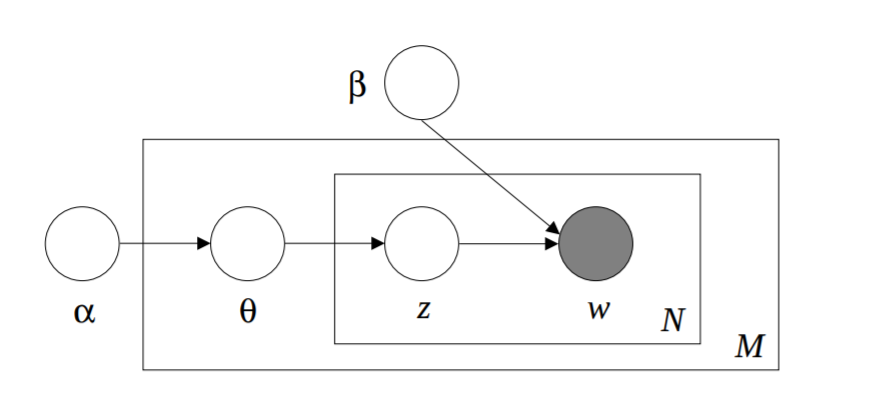
\includegraphics[keepaspectratio=true,scale=0.4]{figuras/lda1.png}
	\caption{Representação gráfica de modelo de LDA. As caixas são "placas" representando réplicas. A placa externa representa documentos, enquanto a placa interna representa a escolha repetida de tópicos e palavras dentro de um documento.}
	Fonte: \cite{blei2003}
	\label{fig:lda}
\end{figure}


O modelo LDA é representado como um modelo gráfico probabilístico na Figura \ref{fig:lda}. Existem três níveis para a representação LDA. Os parâmetros $\alpha$ e $\beta$ são parâmetros de corpus, assumidos como amostrados uma vez no processo de geração de um corpus. As variáveis $\theta_d$ são variáveis no nível do documento, amostradas uma vez por documento. Finalmente, as variáveis $z_{dn}$ e $w_{dn}$ são variáveis no nível da palavra e são amostradas uma vez para cada palavra em cada documento.

%http://conteudo.icmc.usp.br/CMS/Arquivos/arquivos_enviados/BIBLIOTECA_158_RT_409.pdf

%http://www.jmlr.org/papers/volume3/blei03a/blei03a.pdf